% Options for packages loaded elsewhere
\PassOptionsToPackage{unicode}{hyperref}
\PassOptionsToPackage{hyphens}{url}
%
\documentclass[
]{article}
\usepackage{amsmath,amssymb}
\usepackage{lmodern}
\usepackage{ifxetex,ifluatex}
\ifnum 0\ifxetex 1\fi\ifluatex 1\fi=0 % if pdftex
  \usepackage[T1]{fontenc}
  \usepackage[utf8]{inputenc}
  \usepackage{textcomp} % provide euro and other symbols
\else % if luatex or xetex
  \usepackage{unicode-math}
  \defaultfontfeatures{Scale=MatchLowercase}
  \defaultfontfeatures[\rmfamily]{Ligatures=TeX,Scale=1}
\fi
% Use upquote if available, for straight quotes in verbatim environments
\IfFileExists{upquote.sty}{\usepackage{upquote}}{}
\IfFileExists{microtype.sty}{% use microtype if available
  \usepackage[]{microtype}
  \UseMicrotypeSet[protrusion]{basicmath} % disable protrusion for tt fonts
}{}
\makeatletter
\@ifundefined{KOMAClassName}{% if non-KOMA class
  \IfFileExists{parskip.sty}{%
    \usepackage{parskip}
  }{% else
    \setlength{\parindent}{0pt}
    \setlength{\parskip}{6pt plus 2pt minus 1pt}}
}{% if KOMA class
  \KOMAoptions{parskip=half}}
\makeatother
\usepackage{xcolor}
\IfFileExists{xurl.sty}{\usepackage{xurl}}{} % add URL line breaks if available
\IfFileExists{bookmark.sty}{\usepackage{bookmark}}{\usepackage{hyperref}}
\hypersetup{
  pdftitle={SPAN Stage One Report - Early vs Late Metrics},
  pdfauthor={Ryan P. Cabeen, Cenk Ayata, and SPAN},
  hidelinks,
  pdfcreator={LaTeX via pandoc}}
\urlstyle{same} % disable monospaced font for URLs
\usepackage[margin=1in]{geometry}
\usepackage{graphicx}
\makeatletter
\def\maxwidth{\ifdim\Gin@nat@width>\linewidth\linewidth\else\Gin@nat@width\fi}
\def\maxheight{\ifdim\Gin@nat@height>\textheight\textheight\else\Gin@nat@height\fi}
\makeatother
% Scale images if necessary, so that they will not overflow the page
% margins by default, and it is still possible to overwrite the defaults
% using explicit options in \includegraphics[width, height, ...]{}
\setkeys{Gin}{width=\maxwidth,height=\maxheight,keepaspectratio}
% Set default figure placement to htbp
\makeatletter
\def\fps@figure{htbp}
\makeatother
\setlength{\emergencystretch}{3em} % prevent overfull lines
\providecommand{\tightlist}{%
  \setlength{\itemsep}{0pt}\setlength{\parskip}{0pt}}
\setcounter{secnumdepth}{-\maxdimen} % remove section numbering
\usepackage{booktabs}
\usepackage{makecell}
\ifluatex
  \usepackage{selnolig}  % disable illegal ligatures
\fi

\title{SPAN Stage One Report - Early vs Late Metrics}
\author{Ryan P. Cabeen, Cenk Ayata, and SPAN}
\date{2021-06-09}

\begin{document}
\maketitle

This report investigates the relationship between early timepoint lesion
volume and late timepoint atropy. We examine the general relationship
and further refine the analysis by accounting for inter-site differences
and also by refining the analysis to look at hemisphere-specific atropy
measures.

\newpage

\hypertarget{does-early-timepoint-lesion-predict-late-timepoint-atropy}{%
\section{Does early timepoint lesion predict late timepoint
atropy?}\label{does-early-timepoint-lesion-predict-late-timepoint-atropy}}

An initial test shows a strong relationship between early timepoint and
late tissue volume (whole brain). There are clearly inter-site
differences in total brain volume at the late timepoint, so let's
incorporate that into the model and see how that improves things.

\begin{center}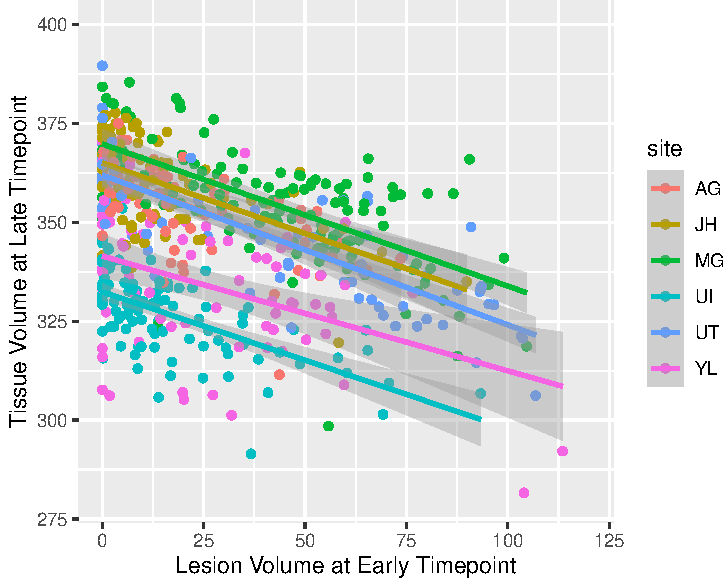
\includegraphics{paper_files/figure-latex/plot_raw-1} \end{center}

\begin{verbatim}
## 
## Call:
## lm(formula = late_tissue ~ early_lesion, data = compare.df)
## 
## Residuals:
##     Min      1Q  Median      3Q     Max 
## -52.641 -12.814   3.453  12.775  36.064 
## 
## Coefficients:
##               Estimate Std. Error t value Pr(>|t|)    
## (Intercept)  353.48784    0.98924 357.332   <2e-16 ***
## early_lesion  -0.25597    0.02617  -9.782   <2e-16 ***
## ---
## Signif. codes:  0 '***' 0.001 '**' 0.01 '*' 0.05 '.' 0.1 ' ' 1
## 
## Residual standard error: 17.06 on 575 degrees of freedom
## Multiple R-squared:  0.1427, Adjusted R-squared:  0.1412 
## F-statistic: 95.68 on 1 and 575 DF,  p-value: < 2.2e-16
\end{verbatim}

\hypertarget{when-we-correct-for-inter-site-differences-how-does-early-timepoint-lesion-predict-late-timepoint-atropy}{%
\section{When we correct for inter-site differences, how does early
timepoint lesion predict late timepoint
atropy?}\label{when-we-correct-for-inter-site-differences-how-does-early-timepoint-lesion-predict-late-timepoint-atropy}}

We see that the inter-site differences are a major source of variance,
and simplying adding the site as a covariate improves the model
dramatically, increasing the R2 from 0.142 to 0.67. The slopes look
similar, but next, let's check that by adding interaction by site.

\begin{center}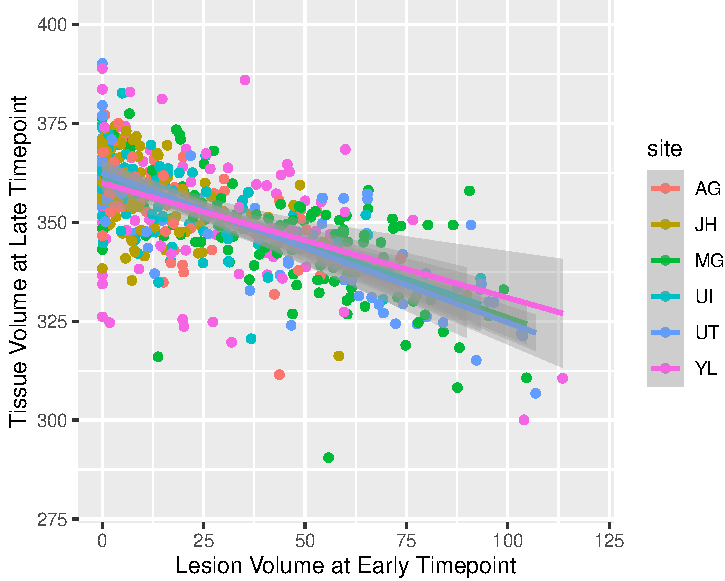
\includegraphics{paper_files/figure-latex/plot_harm-1} \end{center}

\begin{verbatim}
## 
## Call:
## lm(formula = late_tissue ~ early_lesion + site, data = compare.df)
## 
## Residuals:
##     Min      1Q  Median      3Q     Max 
## -51.343  -5.983   0.834   6.763  36.831 
## 
## Coefficients:
##               Estimate Std. Error t value Pr(>|t|)    
## (Intercept)  361.65106    1.21191 298.415  < 2e-16 ***
## early_lesion  -0.35549    0.01816 -19.578  < 2e-16 ***
## siteJH         3.32887    1.56177   2.131   0.0335 *  
## siteMG         7.96041    1.55819   5.109 4.43e-07 ***
## siteUI       -29.09954    1.54481 -18.837  < 2e-16 ***
## siteUT        -0.58592    1.68993  -0.347   0.7289    
## siteYL       -18.44731    1.69730 -10.869  < 2e-16 ***
## ---
## Signif. codes:  0 '***' 0.001 '**' 0.01 '*' 0.05 '.' 0.1 ' ' 1
## 
## Residual standard error: 10.54 on 570 degrees of freedom
## Multiple R-squared:  0.6753, Adjusted R-squared:  0.6719 
## F-statistic: 197.6 on 6 and 570 DF,  p-value: < 2.2e-16
\end{verbatim}

\hypertarget{are-there-site-specific-rates-for-early-timepoint-lesion-predict-late-timepoint-atropy}{%
\section{Are there site-specific rates for early timepoint lesion
predict late timepoint
atropy?}\label{are-there-site-specific-rates-for-early-timepoint-lesion-predict-late-timepoint-atropy}}

When including the interaction term, the model doesn't improve in
adjusted R2, and non of the interactions are significant, so we can
safely say that all of the sites have a similar relationship between
early timepoint lesion and late timepoint tissue volume.

This analysis has only looked at whole brain tissue volume, so next we
can look at hemisphere-specific effects.

\begin{verbatim}
## 
## Call:
## lm(formula = late_tissue ~ early_lesion * site, data = compare.df)
## 
## Residuals:
##     Min      1Q  Median      3Q     Max 
## -51.297  -6.006   0.788   7.050  36.296 
## 
## Coefficients:
##                       Estimate Std. Error t value Pr(>|t|)    
## (Intercept)         362.101092   1.611339 224.721  < 2e-16 ***
## early_lesion         -0.379765   0.059942  -6.336 4.83e-10 ***
## siteJH                2.888917   2.061954   1.401  0.16175    
## siteMG                7.667492   2.423117   3.164  0.00164 ** 
## siteUI              -29.708792   2.104365 -14.118  < 2e-16 ***
## siteUT               -0.249971   2.349678  -0.106  0.91531    
## siteYL              -20.662513   2.430296  -8.502  < 2e-16 ***
## early_lesion:siteJH   0.023423   0.088179   0.266  0.79062    
## early_lesion:siteMG   0.020624   0.069918   0.295  0.76812    
## early_lesion:siteUI   0.034135   0.081555   0.419  0.67570    
## early_lesion:siteUT   0.004384   0.067781   0.065  0.94846    
## early_lesion:siteYL   0.089742   0.077910   1.152  0.24986    
## ---
## Signif. codes:  0 '***' 0.001 '**' 0.01 '*' 0.05 '.' 0.1 ' ' 1
## 
## Residual standard error: 10.57 on 565 degrees of freedom
## Multiple R-squared:  0.6766, Adjusted R-squared:  0.6703 
## F-statistic: 107.5 on 11 and 565 DF,  p-value: < 2.2e-16
\end{verbatim}

\newpage

\hypertarget{looking-at-only-the-isilateral-hemisphere-how-does-early-timepoint-lesion-predict-late-timepoint-atropy}{%
\section{Looking at only the isilateral hemisphere, how does early
timepoint lesion predict late timepoint
atropy?}\label{looking-at-only-the-isilateral-hemisphere-how-does-early-timepoint-lesion-predict-late-timepoint-atropy}}

Looking first at the hemisphere ipsilateral to the lesion, we found a
similar trend, but with an increased R2. What about again controlling
for inter-site differences?

\begin{center}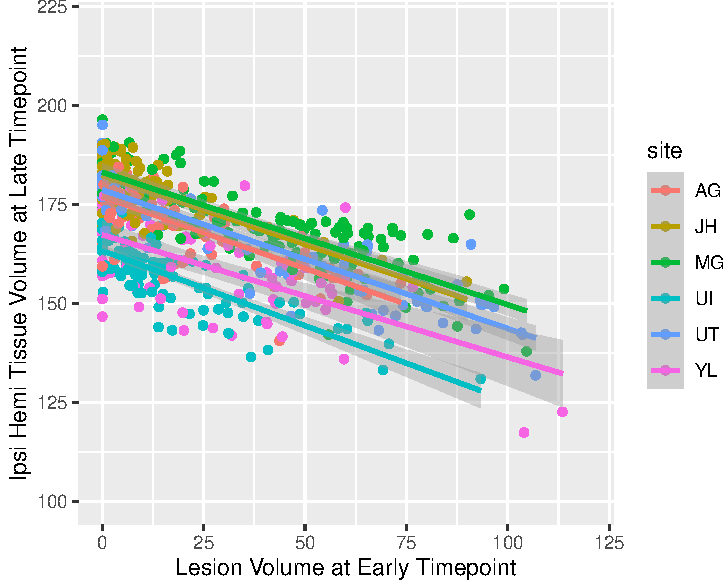
\includegraphics{paper_files/figure-latex/plot_raw_ipsi-1} \end{center}

\begin{verbatim}
## 
## Call:
## lm(formula = late_midline_right ~ early_lesion, data = compare.df)
## 
## Residuals:
##     Min      1Q  Median      3Q     Max 
## -27.694  -7.156   1.559   7.427  24.409 
## 
## Coefficients:
##               Estimate Std. Error t value Pr(>|t|)    
## (Intercept)  174.35212    0.58773  296.65   <2e-16 ***
## early_lesion  -0.29053    0.01555  -18.69   <2e-16 ***
## ---
## Signif. codes:  0 '***' 0.001 '**' 0.01 '*' 0.05 '.' 0.1 ' ' 1
## 
## Residual standard error: 10.13 on 575 degrees of freedom
## Multiple R-squared:  0.3778, Adjusted R-squared:  0.3768 
## F-statistic: 349.2 on 1 and 575 DF,  p-value: < 2.2e-16
\end{verbatim}

\hypertarget{looking-at-only-the-isilateral-hemisphere-and-controlling-for-inter-site-differences-how-does-early-timepoint-lesion-predict-late-timepoint-atropy}{%
\section{Looking at only the isilateral hemisphere and controlling for
inter-site differences, how does early timepoint lesion predict late
timepoint
atropy?}\label{looking-at-only-the-isilateral-hemisphere-and-controlling-for-inter-site-differences-how-does-early-timepoint-lesion-predict-late-timepoint-atropy}}

Again, we find that inter-site differences in brain volume are a major
contributor to the variance, but a covariate can control this quite
well. The overall R2 has increased from 0.67 to 0.73. Next, let's look
at the side contralateral to the lesion.

\begin{center}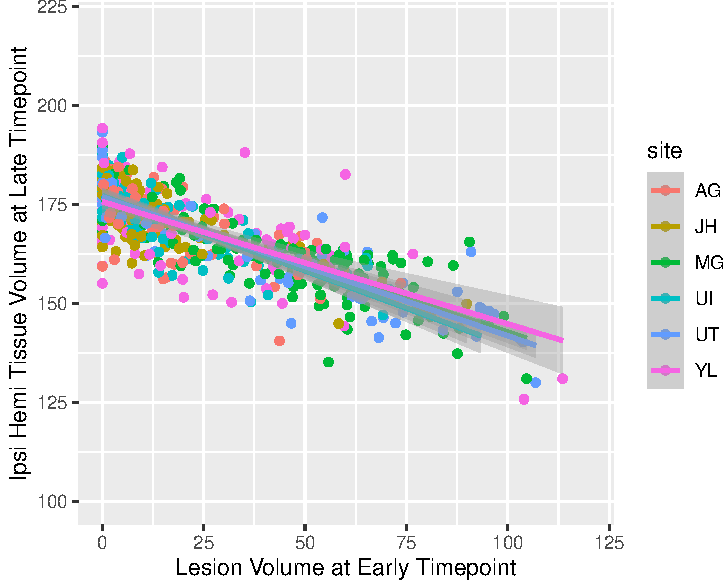
\includegraphics{paper_files/figure-latex/plot_harm_ipsi-1} \end{center}

\begin{verbatim}
## 
## Call:
## lm(formula = late_midline_right ~ early_lesion + site, data = compare.df)
## 
## Residuals:
##      Min       1Q   Median       3Q      Max 
## -22.2702  -4.1505   0.6929   4.4052  26.5940 
## 
## Coefficients:
##               Estimate Std. Error t value Pr(>|t|)    
## (Intercept)  176.65503    0.76201 231.827  < 2e-16 ***
## early_lesion  -0.34464    0.01142 -30.186  < 2e-16 ***
## siteJH         5.62748    0.98200   5.731 1.62e-08 ***
## siteMG         6.91200    0.97975   7.055 5.03e-12 ***
## siteUI       -13.89266    0.97133 -14.303  < 2e-16 ***
## siteUT         1.83998    1.06258   1.732   0.0839 .  
## siteYL        -8.38589    1.06721  -7.858 1.96e-14 ***
## ---
## Signif. codes:  0 '***' 0.001 '**' 0.01 '*' 0.05 '.' 0.1 ' ' 1
## 
## Residual standard error: 6.629 on 570 degrees of freedom
## Multiple R-squared:  0.7361, Adjusted R-squared:  0.7333 
## F-statistic:   265 on 6 and 570 DF,  p-value: < 2.2e-16
\end{verbatim}

\hypertarget{looking-at-only-the-contralateral-hemisphere-how-does-early-timepoint-lesion-predict-late-timepoint-atropy}{%
\section{Looking at only the contralateral hemisphere, how does early
timepoint lesion predict late timepoint
atropy?}\label{looking-at-only-the-contralateral-hemisphere-how-does-early-timepoint-lesion-predict-late-timepoint-atropy}}

When looking at tissue volume on the hemisphere contralateral to the
lesion, we see that there is now no relation relationship between early
timepoint lesion volume and late timepoint tissue volume, suggesting
that the atrophy is localized to the ispilateral side.

\begin{center}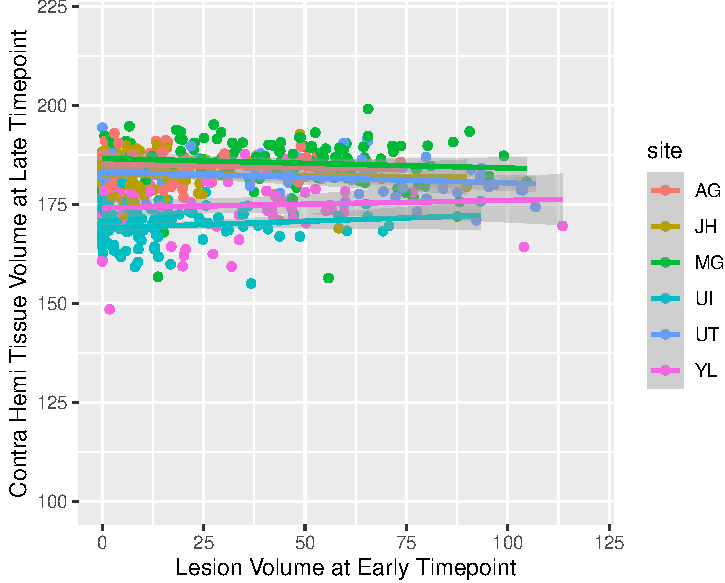
\includegraphics{paper_files/figure-latex/plot_raw_contra-1} \end{center}

\begin{verbatim}
## 
## Call:
## lm(formula = late_midline_left ~ early_lesion, data = compare.df)
## 
## Residuals:
##     Min      1Q  Median      3Q     Max 
## -30.679  -5.455   1.458   5.771  17.728 
## 
## Coefficients:
##               Estimate Std. Error t value Pr(>|t|)    
## (Intercept)  179.13574    0.45844  390.75  < 2e-16 ***
## early_lesion   0.03456    0.01213    2.85  0.00453 ** 
## ---
## Signif. codes:  0 '***' 0.001 '**' 0.01 '*' 0.05 '.' 0.1 ' ' 1
## 
## Residual standard error: 7.904 on 575 degrees of freedom
## Multiple R-squared:  0.01393,    Adjusted R-squared:  0.01221 
## F-statistic: 8.121 on 1 and 575 DF,  p-value: 0.004533
\end{verbatim}

\hypertarget{looking-at-only-the-contralateral-hemisphere-and-controlling-for-inter-site-differences-how-does-early-timepoint-lesion-predict-late-timepoint-atropy}{%
\section{Looking at only the contralateral hemisphere and controlling
for inter-site differences, how does early timepoint lesion predict late
timepoint
atropy?}\label{looking-at-only-the-contralateral-hemisphere-and-controlling-for-inter-site-differences-how-does-early-timepoint-lesion-predict-late-timepoint-atropy}}

We further confirm this finding by including a covariate for site.

\begin{center}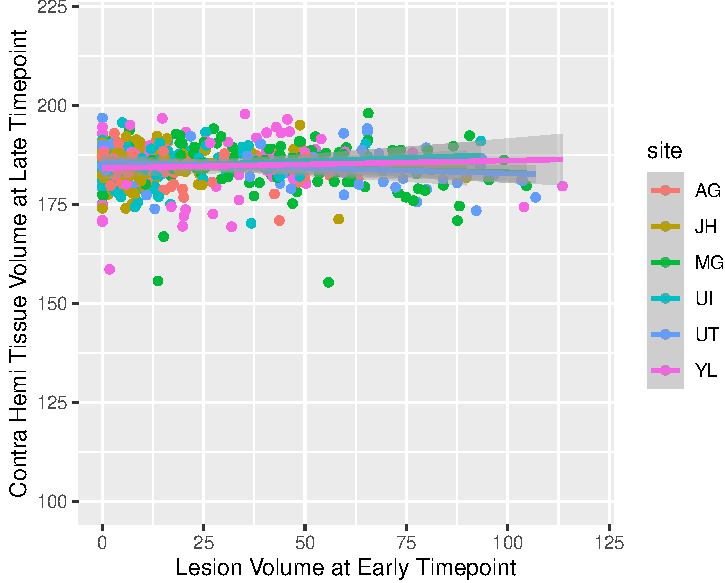
\includegraphics{paper_files/figure-latex/plot_harm_contra-1} \end{center}

\begin{verbatim}
## 
## Call:
## lm(formula = late_midline_left ~ early_lesion + site, data = compare.df)
## 
## Residuals:
##      Min       1Q   Median       3Q      Max 
## -29.1733  -2.6685   0.4958   3.2167  13.7973 
## 
## Coefficients:
##                Estimate Std. Error t value Pr(>|t|)    
## (Intercept)  184.996033   0.603696 306.439  < 2e-16 ***
## early_lesion  -0.010852   0.009045  -1.200  0.23071    
## siteJH        -2.298580   0.777977  -2.955  0.00326 ** 
## siteMG         1.048370   0.776193   1.351  0.17734    
## siteUI       -15.206833   0.769525 -19.761  < 2e-16 ***
## siteUT        -2.425874   0.841816  -2.882  0.00410 ** 
## siteYL       -10.061479   0.845485 -11.900  < 2e-16 ***
## ---
## Signif. codes:  0 '***' 0.001 '**' 0.01 '*' 0.05 '.' 0.1 ' ' 1
## 
## Residual standard error: 5.252 on 570 degrees of freedom
## Multiple R-squared:  0.5685, Adjusted R-squared:  0.564 
## F-statistic: 125.2 on 6 and 570 DF,  p-value: < 2.2e-16
\end{verbatim}

\end{document}
